% ==========================================================
% SYSTEM TESTING & AUTOMATED SELENIUM TEST RESULTS
% ==========================================================

Testing was performed at different levels to identify functional and integration errors. Unit testing focused on individual utility and DAO operations, integration testing verified communication between JSP pages, servlets, DAO classes, and the MySQL database, while validation testing checked system responses to invalid inputs. Selenium WebDriver was also used for automated end-to-end testing.

\subsection{Unit Testing}
Unit testing was used to verify individual components of the application before complete system integration. Important components such as password hashing and verification, skill creation through form inputs, rating operations, saved-skill operations, and input validation were checked using valid and invalid inputs.

\vspace{0.3cm}
\noindent\textit{Unit Test Execution Summary}
\vspace{0.2cm}

\begin{table}[H]
\centering
\small
\begin{tabularx}{\textwidth}{|L{2.0cm}|L{4.0cm}|L{4.8cm}|L{2.0cm}|}
\hline
\textbf{Test ID} & \textbf{Test Description} & \textbf{Expected Output} & \textbf{Status} \\ \hline
UT-01 & Password hashing and verification & Correct password is verified successfully & Passed \\ \hline
UT-02 & Skill creation through SkillDAO & Valid skill details are stored in database & Passed \\ \hline
UT-03 & Rating validation & Only ratings from 1 to 5 are accepted & Passed \\ \hline
UT-04 & Saved-skill operation & Skill course is correctly added & Passed \\ \hline
UT-05 & Price validation & Invalid or negative prices are rejected & Passed \\ \hline
\end{tabularx}
\end{table}

\subsection{Integration Testing}
Integration testing verified the complete communication between the presentation, servlet, DAO, and database layers. For example, submitting the Add Skill form was tested to confirm that the servlet receives the data, validates it, passes it to the database, and stores the resulting record in the MySQL database. Similarly, ratings, saved skills, and browse operations were checked from the user interface through the database.

\vspace{0.3cm}
\noindent\textit{Integration Test Results}
\vspace{0.2cm}

\begin{table}[H]
\centering
\small
\begin{tabularx}{\textwidth}{|L{1.8cm}|L{3.8cm}|L{5.0cm}|L{2.0cm}|}
\hline
\textbf{ID} & \textbf{Test Case} & \textbf{Expected Result} & \textbf{Status} \\ \hline
VT-01 & Required Fields & Empty required fields are rejected. & Passed \\ \hline
VT-02 & Price Validation & Invalid or zero prices are rejected. & Passed \\ \hline
VT-03 & Duplicate Skill & Duplicate skill courses are detected before insertion. & Passed \\ \hline
VT-04 & Authentication & Restricted operations require user login. & Passed \\ \hline
VT-05 & Rating Range & Only ratings from 1--5 are accepted. & Passed \\ \hline
VT-06 & Duplicate Rating & Duplicate ratings for the same skill are prevented. & Passed \\ \hline
\end{tabularx}
\end{table}

\subsection{User Acceptance Testing}
User acceptance testing was performed to evaluate the overall usability of ElderEarn. Users were asked to perform common tasks such as registering, logging in, searching for skills, viewing course details, publishing new skills, and browsing the marketplace. The testing focused on ease of navigation, clarity of information, responsiveness, and overall user experience for older adults.

\subsection{Validation Testing}
Validation testing was performed to ensure that invalid or incomplete inputs are handled correctly. Required fields in the Add Skill form were checked, invalid prices were rejected, duplicate user entries were detected, and unauthenticated users were prevented from performing restricted operations. Rating values outside the 1--5 range and duplicate ratings for the same skill course were also tested.

\vspace{0.3cm}
\noindent\textit{Validation Test Results}
\vspace{0.2cm}

\begin{table}[H]
\centering
\small
\begin{tabularx}{\textwidth}{|L{1.8cm}|L{3.8cm}|L{5.0cm}|L{2.0cm}|}
\hline
\textbf{ID} & \textbf{Test Case} & \textbf{Expected Result} & \textbf{Status} \\ \hline
VT-01 & Required Fields & Empty required fields are rejected. & Passed \\ \hline
VT-02 & Price Validation & Invalid or zero prices are rejected. & Passed \\ \hline
VT-03 & Duplicate Skill & Duplicate skill courses are detected before insertion. & Passed \\ \hline
VT-04 & Authentication & Restricted operations require user login. & Passed \\ \hline
VT-05 & Rating Range & Only ratings from 1--5 are accepted. & Passed \\ \hline
VT-06 & Duplicate Rating & Duplicate ratings for the same skill are prevented. & Passed \\ \hline
\end{tabularx}
\end{table}

\section{Test Results and Analysis}
The testing activities confirmed that the major ElderEarn functions operate according to their intended requirements. Unit and integration testing helped verify communication between the JSP, Servlet, DAO, and MySQL database layers, while validation testing confirmed that important business rules were enforced. The completed Selenium login test successfully verified the user authentication workflow. Further automated tests can be added to increase test coverage for course contribution, ratings, saved skills, and other user workflows.

\vspace{0.5cm}
\subsection*{1. Login Test Functionality}

\begin{lstlisting}[language=Java, style=codeStyle, numbers=none]
package seleniumtests;

import org.openqa.selenium.By;
import org.openqa.selenium.WebDriver;
import org.openqa.selenium.chrome.ChromeDriver;

public class LoginTest {
    public static void main(String[] args) {
        WebDriver driver = new ChromeDriver();
        try {
            driver.get("http://localhost:8080/ElderEarn/jsp/auth/login.jsp");
            driver.findElement(By.id("email")).sendKeys("sobin88912@gmail.com");
            driver.findElement(By.id("password")).sendKeys("123");
            driver.findElement(By.cssSelector("button[type='submit']")).click();
            Thread.sleep(2000);

            String currentUrl = driver.getCurrentUrl();
            System.out.println("Current URL: " + currentUrl);
            System.out.println();

            if (currentUrl.contains("teacher-dashboard.jsp")) {
                System.out.println("-------------------------");
                System.out.println("Login successful!");
                System.out.println("LOGIN TEST PASSED");
                System.out.println("-------------------------");
            } else {
                System.out.println("LOGIN TEST FAILED");
            }
        } catch (Exception e) {
            System.out.println("LOGIN TEST FAILED");
        }
        driver.quit();
    }
}
\end{lstlisting}

\begin{figure}[H]
\centering
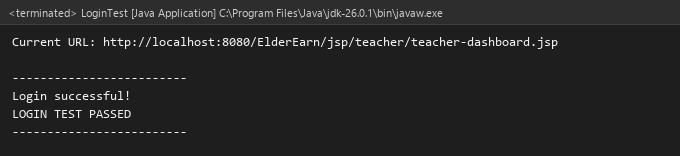
\includegraphics[width=0.78\textwidth]{01_login_test_console.png}
\caption{Login Test Result}
\label{fig:login_test_result}
\end{figure}

\vspace{0.5cm}
\subsection*{2. Add-Skill Test Functionality}

\begin{lstlisting}[language=Java, style=codeStyle, numbers=none]
package seleniumtests;

import java.time.Duration;
import org.openqa.selenium.By;
import org.openqa.selenium.JavascriptExecutor;
import org.openqa.selenium.WebDriver;
import org.openqa.selenium.WebElement;
import org.openqa.selenium.chrome.ChromeDriver;
import org.openqa.selenium.support.ui.ExpectedConditions;
import org.openqa.selenium.support.ui.Select;
import org.openqa.selenium.support.ui.WebDriverWait;

public class AddSkillTest {
    public static void main(String[] args) throws InterruptedException {
        WebDriver driver = new ChromeDriver();
        driver.manage().window().maximize();

        try {
            driver.get("http://localhost:8080/ElderEarn/jsp/auth/login.jsp");
            driver.findElement(By.id("email")).sendKeys("sobin88912@gmail.com");
            driver.findElement(By.id("password")).sendKeys("123");
            driver.findElement(By.cssSelector("button[type='submit']")).click();

            WebDriverWait wait = new WebDriverWait(driver, Duration.ofSeconds(8));
            wait.until(ExpectedConditions.urlContains("teacher-dashboard.jsp"));

            driver.get("http://localhost:8080/ElderEarn/jsp/teacher/add-skill.jsp");
            wait.until(ExpectedConditions.presenceOfElementLocated(By.id("skill_title")));

            driver.findElement(By.id("skill_title")).sendKeys("Organic Kitchen Gardening");
            new Select(driver.findElement(By.id("category"))).selectByValue("Agriculture");
            driver.findElement(By.id("price")).sendKeys("250");
            driver.findElement(By.id("description")).sendKeys("Basics of vermicomposting, soil nutrition, and kitchen gardening.");

            WebElement submitBtn = driver.findElement(By.cssSelector("button[type='submit']"));
            ((JavascriptExecutor) driver).executeScript("arguments[0].scrollIntoView(true);", submitBtn);
            Thread.sleep(500);
            ((JavascriptExecutor) driver).executeScript("arguments[0].click();", submitBtn);

            wait.until(ExpectedConditions.urlContains("view-my-skills.jsp"));

            System.out.println("SKILL ADDED SUCCESSFULLY");
            System.out.println("Enter Skill Title: Organic Kitchen Gardening");
            System.out.println("Enter Category: Agriculture");
            System.out.println("Enter Price: 250");
            System.out.println("Skill Added Successfully");
            System.out.println("ADD SKILL TEST PASSED");
        } catch (Exception e) {
            System.out.println("ADD SKILL TEST FAILED");
        } finally {
            driver.quit();
        }
    }
}
\end{lstlisting}

\begin{figure}[H]
\centering
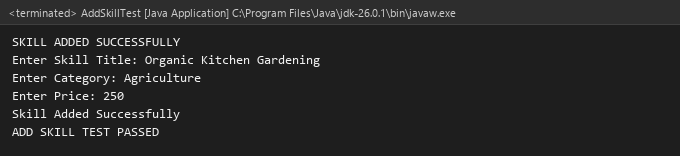
\includegraphics[width=0.78\textwidth]{02_add_skill_test_console.png}
\caption{Add-Skill Test Result}
\label{fig:add_skill_test_result}
\end{figure}

\vspace{0.5cm}
\subsection*{3. Browse-Skills Test Functionality}

\begin{lstlisting}[language=Java, style=codeStyle, numbers=none]
package seleniumtests;

import java.util.List;
import org.openqa.selenium.By;
import org.openqa.selenium.WebDriver;
import org.openqa.selenium.WebElement;
import org.openqa.selenium.chrome.ChromeDriver;

public class BrowseSkillsTest {
    public static void main(String[] args) throws InterruptedException {
        WebDriver driver = new ChromeDriver();

        try {
            driver.get("http://localhost:8080/ElderEarn/jsp/auth/login.jsp");
            driver.findElement(By.id("email")).sendKeys("chu@gmail.com");
            driver.findElement(By.id("password")).sendKeys("123");
            driver.findElement(By.cssSelector("button[type='submit']")).click();
            Thread.sleep(1500);

            driver.get("http://localhost:8080/ElderEarn/jsp/student/browse-skills.jsp");
            Thread.sleep(1500);

            List<WebElement> skillCards = driver.findElements(By.className("skill-card"));
            System.out.println("STUDENT MARKETPLACE LOADED");
            System.out.println("Current URL: " + driver.getCurrentUrl());
            System.out.println("Total Skills Available: " + skillCards.size());

            if (skillCards.size() > 0) {
                System.out.println("-------------------------");
                System.out.println("Skills Catalog Displayed Successfully!");
                System.out.println("BROWSE SKILLS TEST PASSED");
                System.out.println("-------------------------");
            } else {
                System.out.println("BROWSE SKILLS TEST FAILED");
            }
        } catch (Exception e) {
            System.out.println("BROWSE SKILLS TEST FAILED");
        }
        driver.quit();
    }
}
\end{lstlisting}

\begin{figure}[H]
\centering
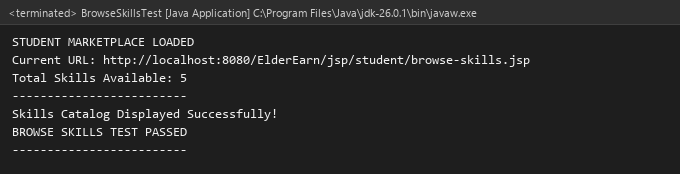
\includegraphics[width=0.78\textwidth]{03_browse_skills_test_console.png}
\caption{Browse-Skills Test Result}
\label{fig:browse_skills_test_result}
\end{figure}